\section{形变收缩核和伦型}
\label{section:ch09-sec58}

我们已经知道, 了解空间 $X$ 的基本群的一个办法便是研究空间 $X$ 的覆叠空间. 另一个办法在这一节中讨论, 涉及伦型概念. 它提供了一种手段, 将计算一个空间的基本群的问题化为计算另一个较为熟悉的空间的基本群.

我们从一个引理开始.

\par
\begin{figure}[htbp]
\centering
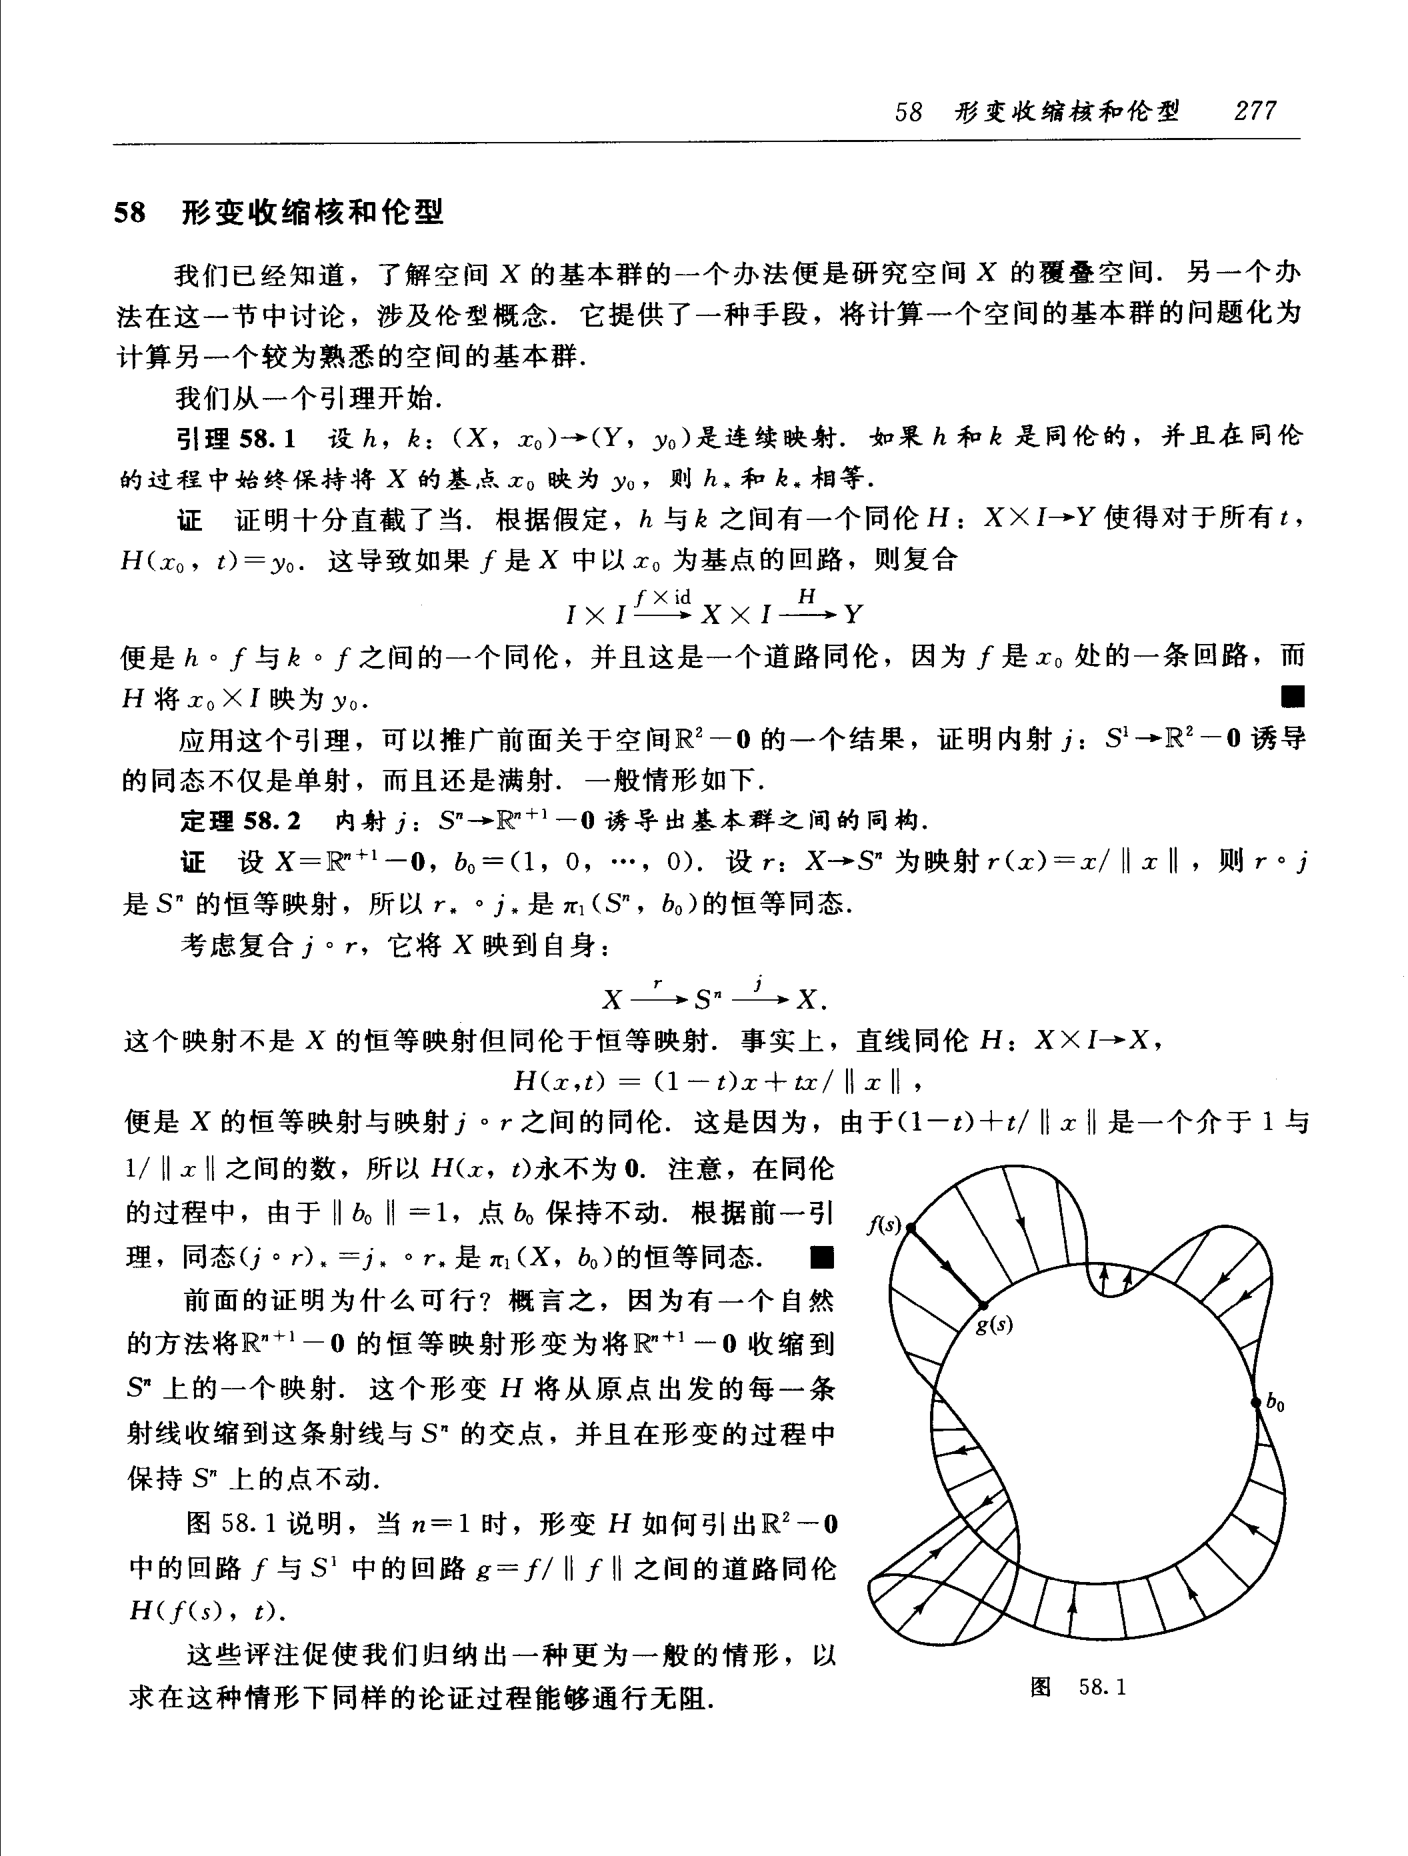
\includegraphics[width=0.5\textwidth]{image/fig-58-1.png}
\caption{形变收缩 $H$.}
\label{figure:ch09-fig-58-1}
\end{figure}

\par
\begin{figure}[htbp]
\centering
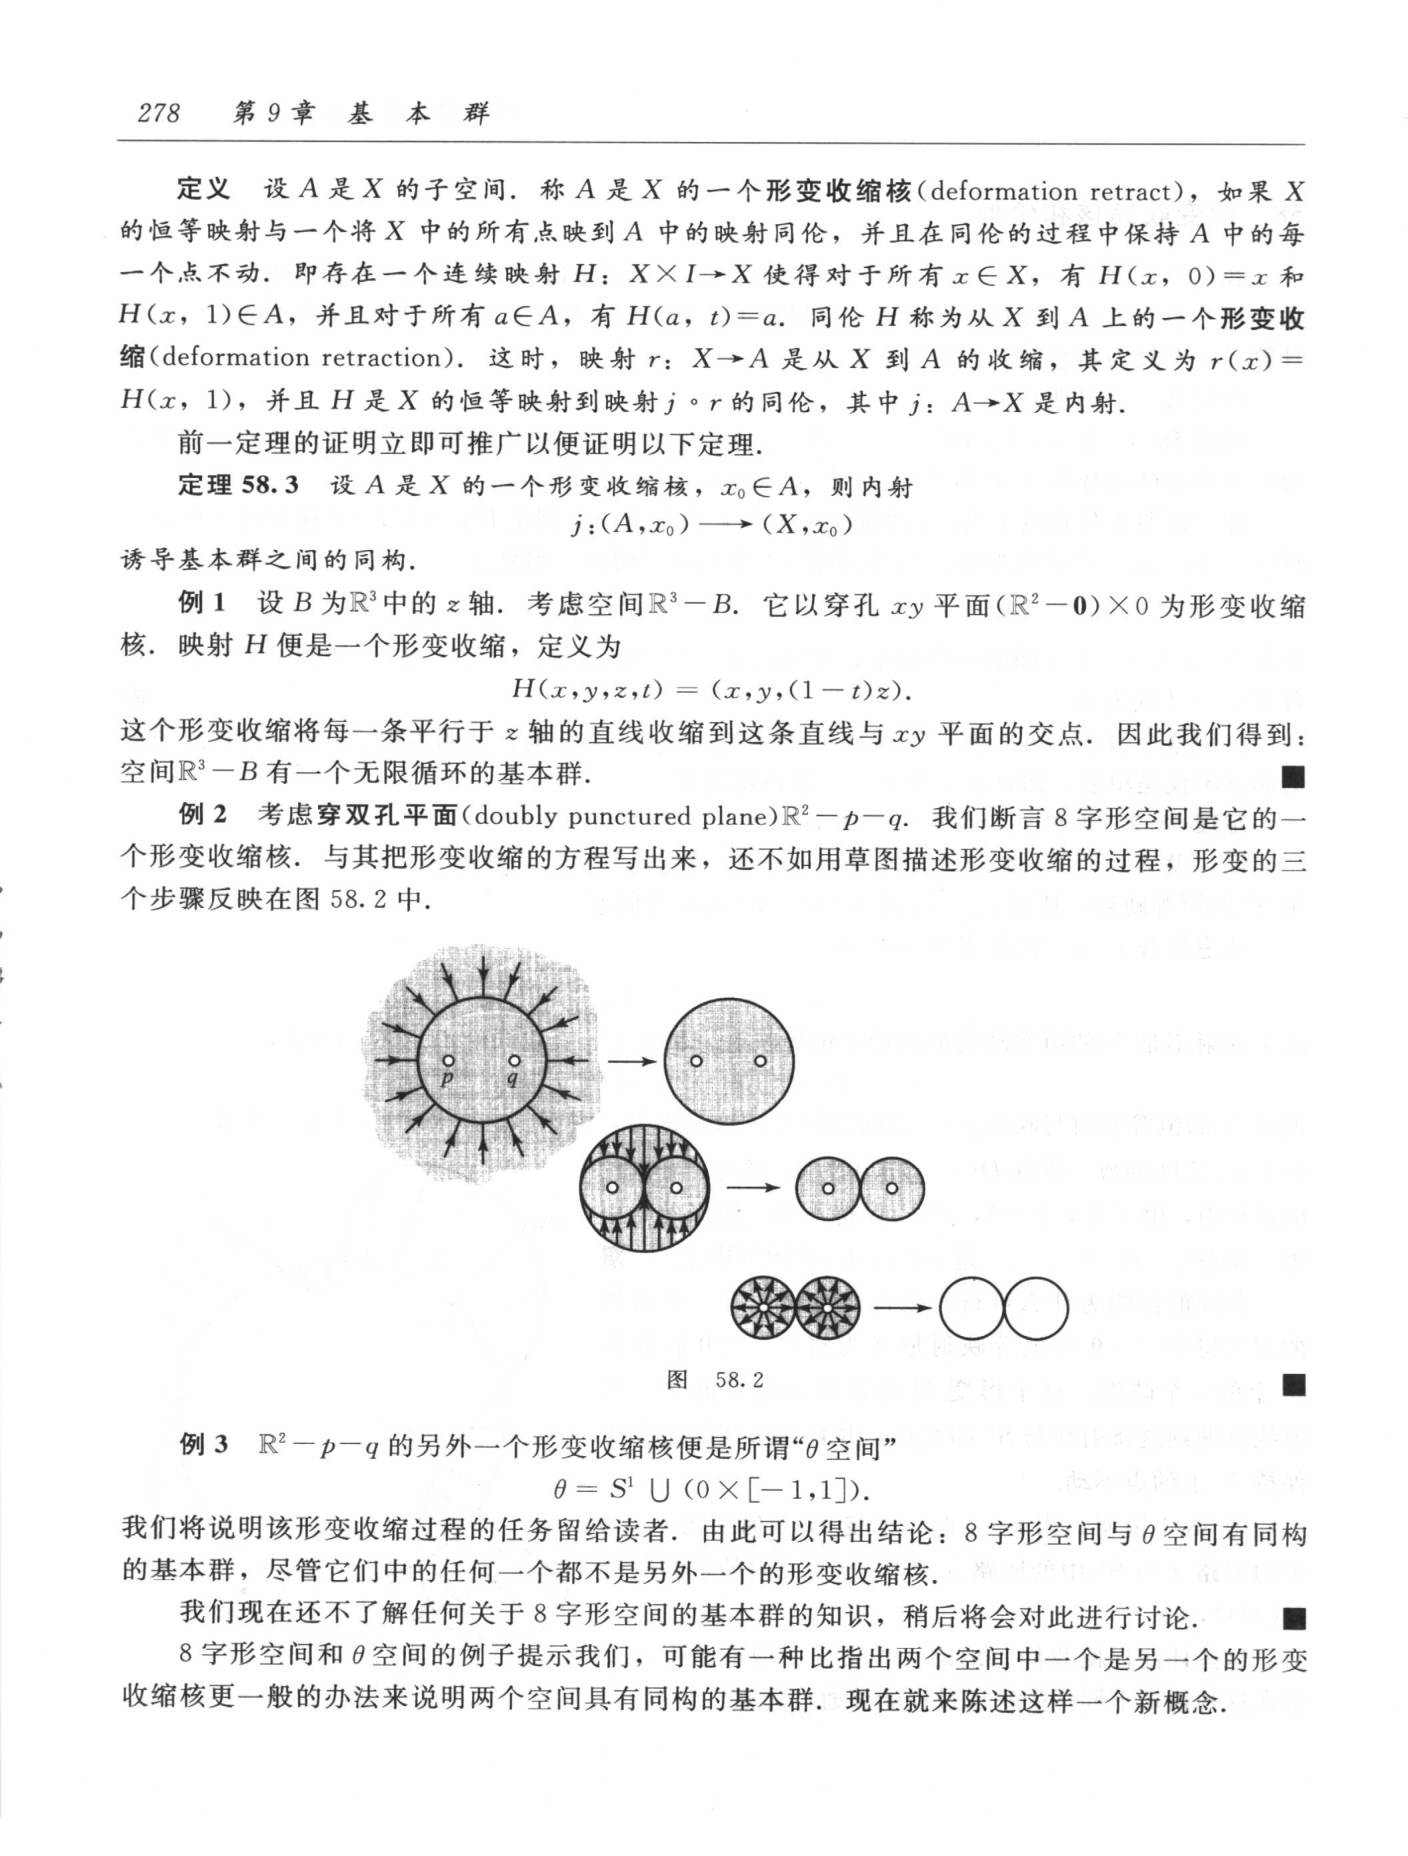
\includegraphics[width=0.6\textwidth]{image/fig-58-2.png}
\caption{穿双孔平面形变收缩到 8 字形空间.}
\label{figure:ch09-fig-58-2}
\end{figure}

\par
\begin{figure}[htbp]
\centering
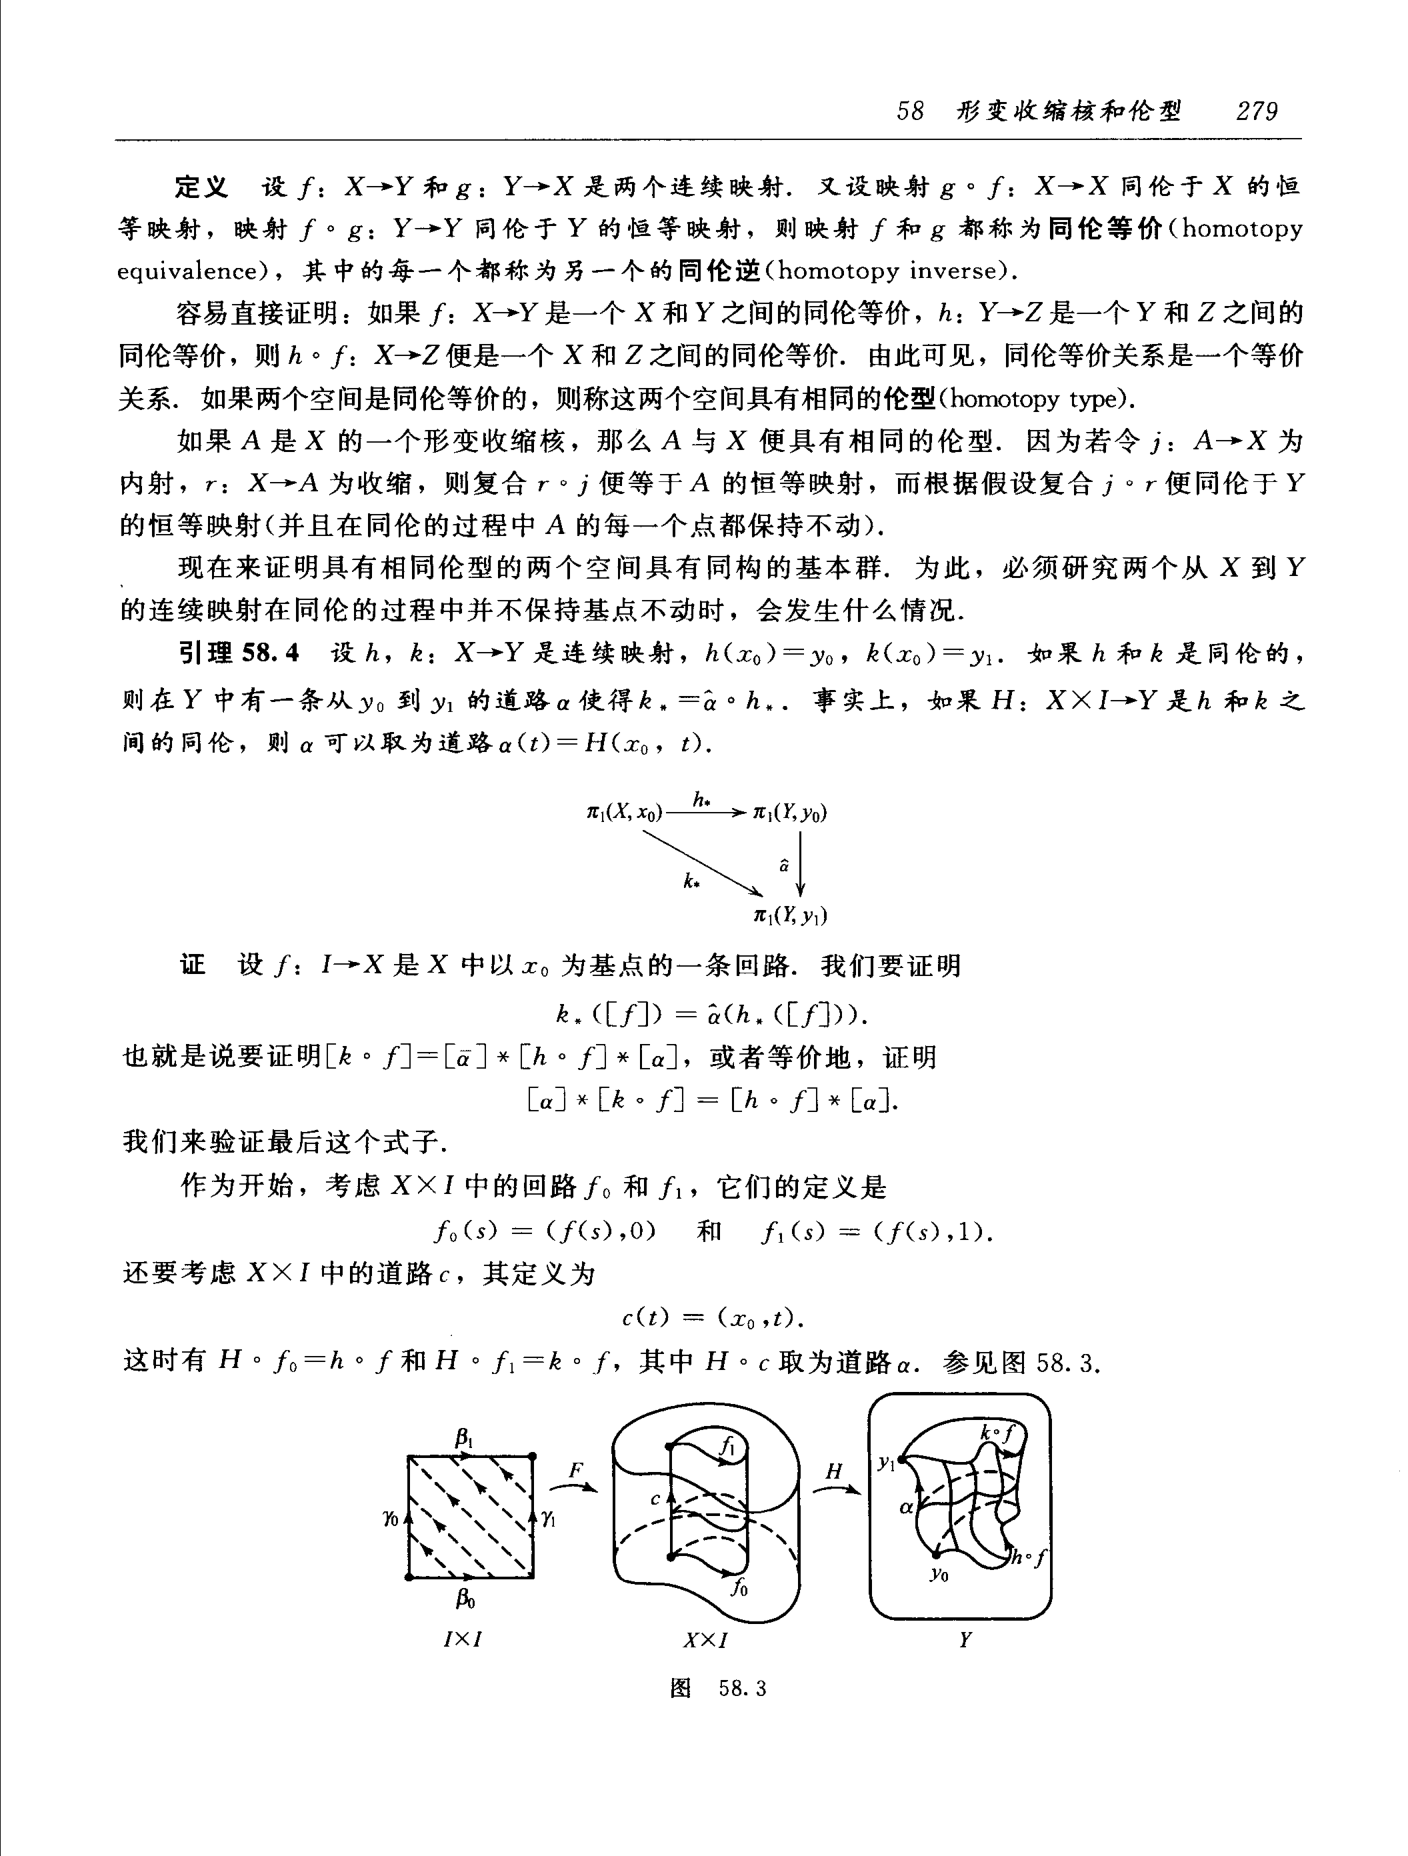
\includegraphics[width=0.7\textwidth]{image/fig-58-3.png}
\caption{引理 \cref{lemma:ch09-sec58-58-4}.}
\label{figure:ch09-fig-58-3}
\end{figure}

\begin{lemma}
\label{lemma:ch09-sec58-58-1}
设 $h,k\colon(X,x_0)\to(Y,y_0)$ 是连续映射. 如果 $h$ 和 $k$ 是同伦的, 并且在同伦的过程中始终保持将 $X$ 的基点 $x_0$ 映为 $y_0$, 则 $h_*$ 和 $k_*$ 相等.
\end{lemma}

\begin{proof}
证明十分直截了当. 根据假定, $h$ 与 $k$ 之间有一个同伦 $H\colon X\times I\to Y$ 使得对于所有 $t$, $H(x_0,t)=y_0$. 这导致如果 $f$ 是 $X$ 中以 $x_0$ 为基点的回路, 则复合
\[
I\times I\xrightarrow{f\times\mathrm{id}}X\times I\xrightarrow{H}Y
\]
便是 $h\circ f$ 与 $k\circ f$ 之间的一个同伦, 并且这是一个道路同伦, 因为 $f$ 是 $x_0$ 处的一条回路, 而 $H$ 将 $x_0\times I$ 映为 $y_0$.
\end{proof}

应用这个引理, 可以推广前面关于空间 $\mathbb{R}^{2}-\boldsymbol{0}$ 的一个结果, 证明内射 $j\colon S^{1}\to\mathbb{R}^{2}-\boldsymbol{0}$ 诱导的同态不仅是单射, 而且还是满射. 一般情形如下.

\begin{theorem}
\label{theorem:ch09-sec58-58-2}
内射 $j\colon S^{n}\to\mathbb{R}^{n+1}-\boldsymbol{0}$ 诱导出基本群之间的同构.
\end{theorem}

\begin{proof}
设 $X=\mathbb{R}^{n+1}-\boldsymbol{0}$, $b_0=(1,0,\cdots,0)$. 设 $r\colon X\to S^{n}$ 为映射 $r(x)=x/\|x\|$, 则 $r\circ j$ 是 $S^{n}$ 的恒等映射, 所以 $r_*\circ j_*$ 是 $\pi_1(S^{n},b_0)$ 的恒等同态.

考虑复合 $j\circ r$, 它将 $X$ 映到自身:
\[
X\xrightarrow{r}S^{n}\xrightarrow{j}X.
\]
这个映射不是 $X$ 的恒等映射但同伦于恒等映射. 事实上, 直线同伦 $H\colon X\times I\to X$,
\[
H(x,t)=(1-t)x+tx/\|x\|,
\]
便是 $X$ 的恒等映射与映射 $j\circ r$ 之间的同伦. 这是因为, 由于 $(1-t)+t/\|x\|$ 是一个介于 $1$ 与 $1/\|x\|$ 之间的数, 所以 $H(x,t)$ 永不为 $\boldsymbol{0}$. 注意, 在同伦的过程中, 由于 $\|b_0\|=1$, 点 $b_0$ 保持不动. 根据前一引理, 同态 $(j\circ r)_*=j_*\circ r_*$ 是 $\pi_1(X,b_0)$ 的恒等同态.
\end{proof}


前面的证明为什么可行? 概言之, 因为有一个自然的方法将 $\mathbb{R}^{n+1}-\boldsymbol{0}$ 的恒等映射形变为将 $\mathbb{R}^{n+1}-\boldsymbol{0}$ 收缩到 $S^{n}$ 上的一个映射. 这个形变 $H$ 将从原点出发的每一条射线收缩到这条射线与 $S^{n}$ 的交点, 并且在形变的过程中保持 $S^{n}$ 上的点不动.

图 \cref{figure:ch09-fig-58-1} 说明, 当 $n=1$ 时, 形变 $H$ 如何引出 $\mathbb{R}^{2}-\boldsymbol{0}$ 中的回路 $f$ 与 $S^{1}$ 中的回路 $g=f/\|f\|$ 之间的道路同伦 $H(f(s),t)$.

这些评注促使我们归纳出一种更为一般的情形, 以求在这种情形下同样的论证过程能够通行无阻.

\begin{definition}[形变收缩核]
\label{definition:ch09-sec58-defretract}
设 $A$ 是 $X$ 的子空间. 称 $A$ 是 $X$ 的一个\textbf{形变收缩核}(deformation retract), 如果 $X$ 的恒等映射与一个将 $X$ 中的所有点映到 $A$ 中的映射同伦, 并且在同伦的过程中保持 $A$ 中的每一个点不动. 即存在一个连续映射 $H\colon X\times I\to X$ 使得对于所有 $x\in X$, 有 $H(x,0)=x$ 和 $H(x,1)\in A$, 并且对于所有 $a\in A$, 有 $H(a,t)=a$. 同伦 $H$ 称为从 $X$ 到 $A$ 上的一个\textbf{形变收缩}(deformation retraction). 这时, 映射 $r\colon X\to A$ 是从 $X$ 到 $A$ 的收缩, 其定义为 $r(x)=H(x,1)$, 并且 $H$ 是 $X$ 的恒等映射到映射 $j\circ r$ 的同伦, 其中 $j\colon A\to X$ 是内射.
\end{definition}

前一定理的证明立即可推广以便证明以下定理.

\begin{theorem}
\label{theorem:ch09-sec58-58-3}
设 $A$ 是 $X$ 的一个形变收缩核, $x_0\in A$, 则内射
\[
j\colon(A,x_{0})\longrightarrow(X,x_{0})
\]
诱导基本群之间的同构.
\end{theorem}

\begin{example}
\label{example:ch09-sec58-1}
设 $B$ 为 $\mathbb{R}^{3}$ 中的 $z$ 轴. 考虑空间 $\mathbb{R}^{3}-B$. 它以穿孔 $xy$ 平面 $(\mathbb{R}^{2}-\boldsymbol{0})\times 0$ 为形变收缩核. 映射 $H$ 便是一个形变收缩, 定义为
\[
H(x,y,z,t)=(x,y,(1-t)z).
\]
这个形变收缩将每一条平行于 $z$ 轴的直线收缩到这条直线与 $xy$ 平面的交点. 因此我们得到: 空间 $\mathbb{R}^{3}-B$ 有一个无限循环的基本群.
\end{example}

\begin{example}
\label{example:ch09-sec58-2}
考虑穿双孔平面 (doubly punctured plane) $\mathbb{R}^{2}-p-q$. 我们断言 8 字形空间是它的一个形变收缩核. 与其把形变收缩的方程写出来, 还不如用草图描述形变收缩的过程, 形变的三个步骤反映在图 \cref{figure:ch09-fig-58-2} 中.
\end{example}


\begin{example}
\label{example:ch09-sec58-3}
$\mathbb{R}^{2}-p-q$ 的另外一个形变收缩核便是所谓"$\theta$ 空间"
\[
\theta=S^{1}\cup(0\times[-1,1]).
\]
我们将说明该形变收缩过程的任务留给读者. 由此可以得出结论: 8 字形空间与 $\theta$ 空间有同构的基本群, 尽管它们中的任何一个都不是另外一个的形变收缩核.

我们现在还不了解任何关于 8 字形空间的基本群的知识, 稍后将会对此进行讨论.
\end{example}

8 字形空间和 $\theta$ 空间的例子提示我们, 可能有一种比指出两个空间中一个是另一个的形变收缩核更一般的办法来说明两个空间具有同构的基本群. 现在就来陈述这样一个新概念.

\begin{definition}[伦型与同伦等价]
\label{definition:ch09-sec58-homotopy-type}
设 $f\colon X\to Y$ 和 $g\colon Y\to X$ 是两个连续映射. 又设映射 $g\circ f\colon X\to X$ 同伦于 $X$ 的恒等映射, 映射 $f\circ g\colon Y\to Y$ 同伦于 $Y$ 的恒等映射, 则映射 $f$ 和 $g$ 都称为\textbf{同伦等价}(homotopy equivalence), 其中的每一个都称为另一个的\textbf{同伦逆}(homotopy inverse).

容易直接证明: 如果 $f\colon X\to Y$ 是一个 $X$ 和 $Y$ 之间的同伦等价, $h\colon Y\to Z$ 是一个 $Y$ 和 $Z$ 之间的同伦等价, 则 $h\circ f\colon X\to Z$ 便是一个 $X$ 和 $Z$ 之间的同伦等价. 由此可见, 同伦等价关系是一个等价关系. 如果两个空间是同伦等价的, 则称这两个空间具有相同的\textbf{伦型}(homotopy type).

如果 $A$ 是 $X$ 的一个形变收缩核, 那么 $A$ 与 $X$ 便具有相同的伦型. 因为若令 $j\colon A\to X$ 为内射, $r\colon X\to A$ 为收缩, 则复合 $r\circ j$ 便等于 $A$ 的恒等映射, 而根据假设复合 $j\circ r$ 便同伦于 $Y$ 的恒等映射 (并且在同伦的过程中 $A$ 的每一个点都保持不动).
\end{definition}

现在来证明具有相同伦型的两个空间具有同构的基本群. 为此, 必须研究两个从 $X$ 到 $Y$ 的连续映射在同伦的过程中并不保持基点不动时, 会发生什么情况.

\begin{lemma}
\label{lemma:ch09-sec58-58-4}
设 $h,k\colon X\to Y$ 是连续映射, $h(x_0)=y_0$, $k(x_0)=y_1$. 如果 $h$ 和 $k$ 是同伦的, 则在 $Y$ 中有一条从 $y_0$ 到 $y_1$ 的道路 $\alpha$ 使得 $k_*=\hat{\alpha}\circ h_*$. 事实上, 如果 $H\colon X\times I\to Y$ 是 $h$ 和 $k$ 之间的同伦, 则 $\alpha$ 可以取为道路 $\alpha(t)=H(x_0,t)$.
\end{lemma}

\[
\begin{array}{ccc}
\pi_{1}(X,x_{0}) & \xrightarrow{h_{*}} & \pi_{1}(Y,y_{0})\\
 & \underset{k_{*}}{\searrow} & \downarrow{\scriptstyle\hat{\alpha}}\\
 & & \pi_{1}(Y,y_{1})
\end{array}
\]


\begin{proof}
设 $f\colon I\to X$ 是 $X$ 中以 $x_0$ 为基点的一条回路. 我们要证明
\[
k_{*}([f])=\hat{\alpha}(h_{*}([f])).
\]
也就是说要证明 $[k\circ f]=[\bar{\alpha}]*[h\circ f]*[\alpha]$, 或者等价地, 证明
\[
[\alpha]*[k\circ f]=[h\circ f]*[\alpha].
\]
我们来验证最后这个式子.

作为开始, 考虑 $X\times I$ 中的回路 $f_0$ 和 $f_1$, 它们的定义是
\[
f_{0}(s)=(f(s),0)\quad\text{和}\quad f_{1}(s)=(f(s),1).
\]
还要考虑 $X\times I$ 中的道路 $c$, 其定义为
\[
c(t)=(x_{0},t).
\]
这时有 $H\circ f_0=h\circ f$ 和 $H\circ f_1=k\circ f$, 其中 $H\circ c$ 取为道路 $\alpha$. 参见图 \cref{figure:ch09-fig-58-3}.


设 $F\colon I\times I\to X\times I$ 为映射 $F(s,t)=(f(s),t)$. 考虑 $I\times I$ 中沿着四条边跑的道路:
\[
\beta_{0}(s)=(s,0)\quad\text{和}\quad\beta_{1}(s)=(s,1),\qquad
\gamma_{0}(t)=(0,t)\quad\text{和}\quad\gamma_{1}(t)=(1,t),
\]
这时有 $F\circ\beta_0=f_0$ 和 $F\circ\beta_1=f_1$, 同时 $F\circ\gamma_0=F\circ\gamma_1=c$.

折线道路 $\beta_0*\gamma_1$ 和 $\gamma_0*\beta_1$ 是 $I\times I$ 中从 $(0,0)$ 到 $(1,1)$ 的道路. 由于 $I\times I$ 是凸的, 两者之间有一个道路同伦 $G$. 于是 $F\circ G$ 是 $X\times I$ 中 $f_0*c$ 和 $c*f_1$ 之间的一个道路同伦. 并且 $H\circ(F\circ G)$ 是 $Y$ 中
\[
(H\circ f_{0})*(H\circ c)=(h\circ f)*\alpha
\]
和
\[
(H\circ c)*(H\circ f_{1})=\alpha*(k\circ f)
\]
之间的一个道路同伦. 证毕.
\end{proof}

\begin{corollary}
\label{corollary:ch09-sec58-58-5}
设 $h,k\colon X\to Y$ 是两个同伦的连续映射, $h(x_0)=y_0$, $k(x_0)=y_1$. 如果 $h_*$ 是单射、满射或者平凡的映射, 则 $k_*$ 也相应地是单射、满射或者平凡的映射.
\end{corollary}

\begin{corollary}
\label{corollary:ch09-sec58-58-6}
设 $h\colon X\to Y$. 如果 $h$ 是零伦的, 则 $h_*$ 是平凡的同态.
\end{corollary}

\begin{proof}
常值映射诱导平凡的同态.
\end{proof}

\begin{theorem}
\label{theorem:ch09-sec58-58-7}
设 $f\colon X\to Y$ 是连续的, $f(x_0)=y_0$. 如果 $f$ 是同伦等价, 则
\[
f_{*}\colon\pi_{1}(X,x_{0})\longrightarrow\pi_{1}(Y,y_{0})
\]
是同构.
\end{theorem}

\begin{proof}
设 $g\colon Y\to X$ 是 $f$ 的同伦逆. 考虑映射
\[
(X,x_{0})\xrightarrow{f}(Y,y_{0})\xrightarrow{g}(X,x_{1})\xrightarrow{f}(Y,y_{1}),
\]
其中 $x_1=g(y_0)$, $y_1=f(x_1)$. 我们有相应的诱导同态
\[
\begin{array}{ccc}
\pi_{1}(X,x_{0}) & \xrightarrow{(f_{x_{0}})_{*}} & \pi_{1}(Y,y_{0})\\
 & \underset{g_{*}}{\nearrow} & \downarrow{\scriptstyle(f_{x_{1}})_{*}}\\
\pi_{1}(X,x_{1}) & \xrightarrow{} & \pi_{1}(Y,y_{1})
\end{array}
\]
(这里, 必须区别 $f$ 相对于不同的基点的两个诱导同态.) 根据假定,
\[
g\circ f\colon(X,x_{0})\longrightarrow(X,x_{1})
\]
同伦于恒等映射, 所以 $X$ 中存在道路 $\alpha$ 使得
\[
(g\circ f)_{*}=\hat{\alpha}\circ(i_{X})_{*}=\hat{\alpha}.
\]
这蕴涵着 $(g\circ f)_*=g_*\circ(f_{x_0})_*$ 是同构.

类似地, 由于 $f\circ g$ 同伦于恒等映射 $i_Y$, 同态 $(f\circ g)_*=(f_{x_1})_*\circ g_*$ 也是同构.

前者蕴涵着 $g_*$ 是满射, 后者蕴涵着 $g_*$ 是单射. 因此 $g_*$ 是同构. 再应用一次第一个等式, 可见
\[
(f_{x_{0}})_{*}=(g_{*})^{-1}\circ\hat{\alpha},
\]
所以 $(f_{x_0})_*$ 也是一个同构.

要注意的是, 尽管 $g$ 是 $f$ 的同伦逆, 但同态 $g_*$ 不是同态 $(f_{x_0})_*$ 的逆.
\end{proof}

同伦等价关系明显要比形变收缩的概念更为一般. $\theta$ 空间和 8 字形空间都是穿双孔平面的形变收缩核, 因此它们都同伦等价于穿双孔平面, 所以它们也是相互同伦等价的. 然而其中任何一个都不同胚于另一个的形变收缩核, 事实上每一个都不能嵌入到另一个之中.

令人吃惊的是, 这两个空间发生的状况是典型的. Martin Fuchs 证明了这样一个定理: 两个空间 $X$ 和 $Y$ 同伦等价当且仅当它们分别同胚于同一个空间 $Z$ 的两个形变收缩核. 尽管使用的是初等的工具, 但其证明是困难的 [F].

\subsection*{习题}

\begin{exercise}
证明: 如果 $A$ 是 $X$ 的形变收缩核, $B$ 是 $A$ 的形变收缩核, 则 $B$ 是 $X$ 的形变收缩核.
\end{exercise}

\begin{exercise}
下列空间中的每一个的基本群或者是平凡的, 或者是无限循环群, 或者同构于 8 字形空间的基本群. 试对于每一个空间确定何者成立.
\begin{enumerate}
\item "实心环" $B^{2}\times S^{1}$.
\item 环面 $T$ 挖去一点.
\item 圆柱面 $S^{1}\times I$.
\item 无限的圆柱面 $S^{1}\times\mathbb{R}$.
\item $\mathbb{R}^{3}$ 去掉非负的 $x$, $y$, $z$ 轴.
\end{enumerate}
以下是 $\mathbb{R}^{2}$ 的子集:
\begin{enumerate}
\setcounter{enumi}{5}
\item $\{\,x\mid\|x\|>1\,\}$
\item $\{\,x\mid\|x\|\geqslant 1\,\}$
\item $\{\,x\mid\|x\|<1\,\}$
\item $S^{1}\cup(\mathbb{R}_{+}\times 0)$
\item $S^{1}\cup(\mathbb{R}_{+}\times\mathbb{R})$
\item $S^{1}\cup(\mathbb{R}\times 0)$
\item $\mathbb{R}^{2}-(\mathbb{R}_{+}\times 0)$
\end{enumerate}
\end{exercise}

\begin{exercise}
证明: 对于给定的空间族 $\mathcal{C}$, 同伦等价关系是这个族 $\mathcal{C}$ 上的等价关系.
\end{exercise}

\begin{exercise}
令 $X$ 为 8 字形空间, $Y$ 为 $\theta$ 空间. 描述两个互为同伦逆的映射 $f\colon X\to Y$ 和 $g\colon Y\to X$.
\end{exercise}

\begin{exercise}
复习一个定义: 空间 $X$ 称为\textbf{可缩的}(contractible), 如果 $X$ 到自身的恒等映射是零伦的. 证明: $X$ 是可缩的当且仅当 $X$ 具有一点的伦型.
\end{exercise}

\begin{exercise}
证明: 可缩空间的收缩核是可缩的.
\end{exercise}

\begin{exercise}
设 $A$ 是 $X$ 的子空间, $j\colon A\to X$ 是内射. 又设 $f\colon X\to A$ 是一个连续映射. 假定映射 $j\circ f$ 与 $X$ 的恒等映射之间有一个同伦 $H\colon X\times I\to X$.
\begin{enumerate}
\item 证明: 如果 $f$ 是一个收缩, 则 $j_*$ 是同构.
\item 证明: 如果 $H$ 将 $A\times I$ 映到 $A$ 中, 则 $j_*$ 是同构.
\item 给出一个使得 $j_*$ 不是同构的例子.
\end{enumerate}
\end{exercise}

\begin{exercise}
找一个空间 $X$ 和 $X$ 的一个点 $x_0$ 使得内射 $\{x_0\}\to X$ 是一个同伦等价, 但 $\{x_0\}$ 不是 $X$ 的形变收缩核. [提示: 取 $X$ 为 $\mathbb{R}^{2}$ 的子空间, 它是所有线段 $(1/n)\times I$ ($n\in\mathbb{Z}_{+}$)、线段 $0\times I$ 以及线段 $I\times 0$ 的并. 令 $x_0$ 为点 $(0,1)$. 如果 $\{x_0\}$ 是 $X$ 的形变收缩核, 证明: 对于 $x_0$ 的任意邻域 $U$, $U$ 中包含 $x_0$ 的道路连通分支将包含 $x_0$ 的一个邻域.]
\end{exercise}

\begin{exercise}
定义连续映射 $h\colon S^{1}\to S^{1}$ 的\textbf{度}(degree) 如下:
记 $S^{1}$ 中的点 $(1,0)$ 为 $b_0$, 选取无限循环群 $\pi_1(S^{1},b_0)$ 的一个生成元 $\gamma$. 如果 $x_0$ 是 $S^{1}$ 的一
个点, 选取 $S^{1}$ 中的一条从 $b_0$ 到 $x_0$ 的道路 $\alpha$, 并且定义 $\gamma(x_0)=\hat{\alpha}(\gamma)$. 这时, $\gamma(x_0)$ 生成群 $\pi_1(S^{1},x_0)$. 元素 $\gamma(x_0)$ 不依赖道路 $\alpha$ 的选取, 因为 $S^{1}$ 的基本群是一个交换群.

现在, 对于给定的 $h\colon S^{1}\to S^{1}$, 选取 $x_0\in S^{1}$, 令 $h(x_0)=x_1$. 考虑同态
\[
h_{*}\colon\pi_{1}(S^{1},x_{0})\longrightarrow\pi_{1}(S^{1},x_{1}).
\]
由于两个群都是无限循环群, 我们有
\[
h_{*}(\gamma(x_{0}))=d\cdot\gamma(x_{1})\tag{$*$}
\]
对于某一个整数 $d$ 成立. (群的运算写成加法.) 整数 $d$ 称为 $h$ 的\textbf{度}, 记为 $\deg h$. $h$ 的度并不依赖生成元 $\gamma$ 的选取, 选取不同的生成元只会改变等式 $(*)$ 两边的符号.
\begin{enumerate}
\item 证明 $d$ 不依赖于 $x_0$ 的选取.
\item 证明: 如果 $h$, $k\colon S^{1}\to S^{1}$ 是同伦的, 则它们具有相同的度.
\item 证明 $\deg(h\circ k)=(\deg h)\cdot(\deg k)$.
\item 计算常值映射、恒等映射、反射 $\rho(x_1,x_2)=(x_1,-x_2)$ 和映射 $h(z)=z^n$ 的度, 其中 $z$ 是一个复数.
\item 证明: 如果 $h$, $k\colon S^{1}\to S^{1}$ 具有相同的度, 则它们是同伦的.
\end{enumerate}
\end{exercise}

\begin{exercise}
假设对于每一个映射 $h\colon S^{n}\to S^{n}$ 我们指定了一个整数 $\deg h$, 称之为 $h$ 的度, 满足条件:
\begin{enumerate}
\item 同伦的映射具有相同的度.
\item $\deg(h\circ k)=(\deg h)\cdot(\deg k)$.
\item 恒等映射的度为 $1$, 常值映射的度为 $0$, 反射 $\rho(x_1,\cdots,x_{n+1})=(x_1,\cdots,x_n,-x_{n+1})$ 的度为 $-1$.
\end{enumerate}
[可以用代数拓扑的工具构造这个函数. 直观地说, 度 $\deg h$ 表示 $h$ 将 $S^{n}$ 围绕自身卷了几重. 度的正负告诉我们 $h$ 是否保持定向.] 证明:
\begin{enumerate}
\item 不存在收缩 $r\colon B^{n+1}\to S^{n}$.
\item 如果 $h\colon S^{n}\to S^{n}$ 的度异于 $(-1)^{n+1}$, 则 $h$ 有一个不动点. [提示: 证明如果 $h$ 没有不动点, 则 $h$ 同伦于对径映射 $a(x)=-x$.]
\item 如果 $h\colon S^{n}\to S^{n}$ 的度异于 $1$, 则 $h$ 将某点 $x$ 映为它的对径点 $-x$.
\item 如果 $S^{n}$ 有一个非平凡的切向量场 $v$, 则 $n$ 是奇数. [提示: 如果 $v$ 存在, 证明恒等映射同伦于对径映射.]
\end{enumerate}
\end{exercise}